\section{Chapter Overview}
This chapter will cover the network implemented in the course of the project, beginning with the individual \ac{ADPLL}'s composition. A number of attributes for each design will be used to analyse and compare their performance. The impact of some minor architectural changes will also be covered, before the implementation of test network will be described. This chapter will also highlight some pitfalls encountered in the process. The \ac{HDL} Verilog was selected for use in this project due to my prior exposure to that language. 5 MHz was chosen as the target centre frequency for these \ac{ADPLL}s, during initial testing it was discovered that the waveform output via the Digilent Nexys4 development board's \ac{GPIO} ports began to degrade around the 10 MHz mark, preventing accurate analysis.

\section{\acs{ADPLL} Architectures}
Three different architectures of \ac{ADPLL} were implemented in this project for the purposes of testing, and re-use in the future within the research team in \acl{UCD}. Between each design a number of blocks remain constant, as only a single instance of that block was implemented, as variation its design would have negligible impact on the final system. These blocks were the error combiner and frequency divider. The loop filter was implemented both using fractional and integer arithmetic, but as the exact same calculation was performed in both cases there was no impact on the output of the module.

The three architectures chosen for implementation represent a progression from entirely an \ac{FPGA} clock driven system to an \ac{ADPLL} with all components asynchronous with respect to that clock. Therefore the first \ac{ADPLL} design features a clocked oscillator and phase detector, specifically the linear frequency design mentioned in Chapter \ref{chap:3} and the clocked phase detector using a state machine and a bi-directional counter. Skipping over Design 2, the final design used was asynchronous in totality, featuring the \acl{RO} and SigNum/\ac{TDL} phase detector. Design 2 sat between these two, using the \ac{RO} as its oscillator, but retained the clocked phase detector seen in Design 1.

The extensibility of the end product of this project was to the forefront during the design process. Whilst, apart from frequency, there were no guidelines as to what the system should resemble and a number of attributes could be chosen arbitrarily, a future user of this platform could have entirely different requirements or specifications. As such each block was implemented in such a way that changing the number of bits used for a certain signal, the target frequency or swapping between different blocks could be done with the sole requirement of changing Verilog \texttt{localparam}\footnote{A \texttt{localparam} is a constant that cannot be modified in a module instance statement \cite{hdlworks}}s in the module \footnote{Module is the Verilog term for a number of logic elements grouped to provide a certain functionality} in which change was made, which would then propagate to any sub-modules affected. Starting the design process with this in mind was a major benefit at later stages when frequent modifications were being made to test their impact, or when changing between \ac{ADPLL} designs.

\subsection{Generic Components}
As mentioned in the chapter overview, a number of components were used in all \ac{ADPLL}s implemented, as changes in their design would not impact the overall system.
\subsubsection{Error Combiner}
The error combiner in this design had a number of requirements in order to be suitable for use in both a single \ac{ADPLL} as well as a network operating in both uni- and bi-directional modes, alongside modifications which would change the widths of the error signals requiring averaging. The module was implemented on the basis that the \ac{LF} input width would be identical to the phase detector output width.

The error combiner was designed to take in up to four error signals, all of an identical width which defaults to eight, and four weights to apply in the summation process. A weighted summation is performed by multiplying each error signal by the weight and adding the results together. Regardless of the number of input error signals, a division by four is then performed in order to compute the average error, done by shifting the value right by two. In a \ac{HDL}, unlike C programming or similar, a shift requires no computation and is instead implemented by performing a part-selection. As all error signals are two's complemented signed integers, the error combination process is also carried out using signed values. The code implementing the error combiner can be found in \textsc{ErrorCombiner.v}, attached in Appendix \ref{adx:code} Listing \ref{lst:error_combiner}.

\subsubsection{Frequency Divider}
The frequency divider is implemented using ``Divider 2'' from Chapter \ref{chap:3}, as only divisions ratios of 2, 4 and 8 were selected for use in the testing process. For ease of testing, the divider had outputs representing each of these division ratios simultaneously, which could be multiplexed between at runtime if so desired. A fourth output passed the input through unmodified, allowing for the divider to be removed without regeneration of the \ac{FPGA} configuration.
\begin{figure}[h]%
	\centering
	
\includegraphics[width=0.6\textwidth]{../divider2}
	\caption[Frequency divider \ac{RTL} diagram]{Frequency divider \ac{RTL} diagram.}
	\label{fig:divs_iompl}
\end{figure}

\subsubsection{Loop Filter}
Two \acl{LF}s were implemented, both as \ac{IIR} filters. \ac{FIR} was dismissed due to the extra hardware required to implement the calculations within a single clock cycle, as the \ac{LF} is clocked using the oscillator output, and the greater difficulty of gain adjustment compared to an \ac{IIR}. Clocking on using the generated signal ensures that the discrete time integration is only carried out once per phase comparison. A pitfall that may be encountered implementing an \ac{ADPLL} featuring a divider is not clocking the module on the divided clock, which will result in the integration being carried out at the oscillator output frequency.

Each of integer and fixed-point arithmetic were used to implement a filter respectively, however both designs are interchangeable as they perform the integration identically, given the same proportional and integral gains. All testing was carried out using integer arithmetic, as in Figure \ref{fig:integer_lf}, however the interchangeability will be confirmed later in this chapter, in Section \ref{section:minor_variations}. Additionally the \ac{LF} supports variation of both \acs{ki} and \acs{kp} at runtime, however, if a static value is desired the runtime variation may be disabled using a \texttt{parameter}\footnote{Parameters are constant values that may be changed at compile time, or in the module instance statement \cite{hdlworks2}}.
\begin{figure}[h]%
	\centering
	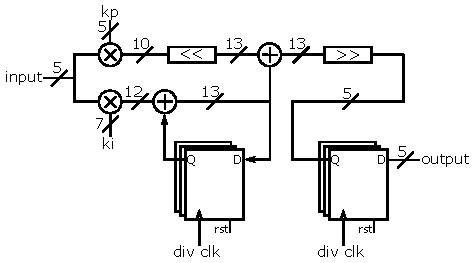
\includegraphics[width=0.8\textwidth]{../integer_lf} 
	\caption[\acl{LF} implemented using integer arithmetic \ac{RTL} diagram]{\acl{LF} implemented using integer arithmetic \ac{RTL} diagram (signal widths using default values).}
	\label{fig:integer_lf}
\end{figure}

Figure \ref{fig:integer_lf} contains an \ac{RTL} diagram describing the implementation. Important to note is the shift applied to the result of the multiplication by \acs{kp} which, as the integration is performed with a larger width to avoid accumulator overflow, preserves the intended relationship between proportional and integral gains.
The Verilog implementation of the \ac{LF} using integer arithmetic can be found in \textsc{LoopFilter.v}, attached in Appendix \ref{adx:code} Listing \ref{lst:loop_filter}.

\subsection{\acs{ADPLL} Design 1}
\acs{ADPLL} Design 1 is comprised of the aforementioned generic components and \ac{FPGA} clocked implementations of the \ac{PFD} and \ac{DCO}. This was the first solution addressed in the course of this project as it is the simplest to both implement and test, as all aspects of the \ac{ADPLL} are driven by the \ac{FPGA} clock. Compared to later designs utilising the \ac{RO}, Vivado simulations could be carried out, with accurate timing behaviour, depicting the locking process. The \ac{DCO} was chosen to be linear in frequency in order to obtain a square wave output as it was not yet known whether the varying pulse width of a period linear design would cause a problem in modules which, at that stage in the project, had not yet been designed. Indeed, a later discarded version of the \ac{FPGA} clocked \ac{PFD} relied on equal low and high times. The \ac{PFD} itself was implemented using a Moore type \ac{FSM} driving a up-down counter to convert the time between rising edges to a digital signal.

\subsubsection{\acl{DCO}}
As the \ac{FPGA} clocked, linear frequency oscillator is based on the use of counters, the first stage in its design was the decisions as to their required widths. The equation given previously is used here, with the control code set to zero in order to obtain the centre frequency, and 5 MHz as the target \ac{DCO} frequency:
\begin{align}
f_{osc} &= f_{FPGA}\times\frac{BIAS+CC}{2^{width}}\\
5\times 10^6 &= f_{FPGA}\times\frac{BIAS}{2^{width}}
\end{align}
This still leaves three parameters undecided: The \ac{FPGA} clock, the bit width of the counter and the bias point. As the \ac{FPGA} clock determines the frequency step of the design, a test counter was implemented initially to determine the maximum frequency at which the timing violations would not occur, at this was determined to be 275 MHz. The equation can then be updated, giving the relationship between bias point and counter width:
\begin{align}
5\times 10^6 &= f_{FPGA}\times\frac{BIAS}{2^{width}}\\
\frac{5}{275} &= \frac{BIAS}{2^{width}}
\end{align}
The maximum value of the counter must also be large enough such that with a bias point that allows for a reasonable range of frequency steps to be added or removed. 
This oscillator was originally designed to allow for 64 control codes either side of the bias, which called for a bias point of 65 or greater.
\begin{align}
\frac{5}{275} &= \frac{65}{2^{width}}\\
2^{width} &= \frac{65\cdot275}{5} = 3575 \\
width &= \left \lceil{\log_2 3575}\right \rceil = 12
\end{align}
From the above equation, the smallest counter that can satisfy this constraint is 12 bits wide, however when testing was carried out using a 275 MHz clock timing violations were discovered by Vivado, resulting \ac{FPGA} clock speed reduction to 258 MHz in order to resolve these violations. The correct bias point could then be calculated as $79$:
\begin{align}
\frac{5}{258} &= \frac{BIAS}{2^{12}}\\
 BIAS &= \left \lfloor{\frac{5\cdot 2^{12}}{258}}\right \rceil = \left \lfloor{\frac{20480}{258}}\right \rceil = 79
\end{align}
The frequency step can now be computed as all parameters have been chosen:
\begin{equation}
f_{step} = \frac{f_{FPGA}}{2^{12}} = 62.988~\si{\kilo\hertz}
\end{equation}
At the target frequency of 5 MHz this corresponds to a change in period of:
\begin{align}
f_{step0} &= 79 \times f_{step} = 79 \times 62.988~\si{\kilo\hertz} = 4.976~\si{\mega\hertz} \\
f_{step1} &= 80 \times f_{step} = 80 \times 62.988~\si{\kilo\hertz} = 5.039~\si{\mega\hertz} \\
T_{step}  &= \frac{1}{f_{step0}} - \frac{1}{f_{step1}} = \frac{1}{4.976\times 10^6} - \frac{1}{5.039\times 10^6} \\
T_{step}  &= 2.5~\si{\nano\second}
\end{align}
From the frequency step, control code range and bias the frequency range of this oscillator can be found:
\begin{align}
f_{osc} &= (BIAS+CC)\times f_{step} = (79+CC)\times 62.988~\si{\kilo\hertz}\\
f_{min} &= (79+CC_{min})\times 62.988~\si{\kilo\hertz} = (79-63)\times 62.988~\si{\kilo\hertz} = 1.008~\si{\mega\hertz}\\
f_{max} &= (79+CC_{max})\times 62.988~\si{\kilo\hertz} = (79+63)\times 62.988~\si{\kilo\hertz} = 8.944~\si{\mega\hertz}
\end{align}

Figure \ref{fig:osc2_impl} contains an \ac{RTL} diagram of this oscillator's implementation. As phase error is a two's complement signed value, its addition to the bias must be carried out using signed arithmetic. Provided the bias is greater than the minimum possible phase error, as has been ensured in this case, the result of this addition is positive signed integer. Being a positive quantity, additional logic performing a conversion from a signed to an unsigned representation is required.
\begin{figure}[h]%
	\centering
	
\includegraphics[width=0.8\textwidth]{../osc2_impl} 
	\caption[\ac{DCO} \ac{RTL} diagram as implemented]{\ac{DCO} \ac{RTL} diagram as implemented.}
	\label{fig:osc2_impl}
\end{figure}

\subsubsection{Phase Detector}
As previously mentioned the \ac{PFD} is also implemented using the \ac{FPGA} clocked approach, with sign detection carried out using a Moore Machine. The state transition diagram given as the example in Chapter \ref{chap:3} is that used to design this sign detector. 
\begin{figure}[h]
	\centering
	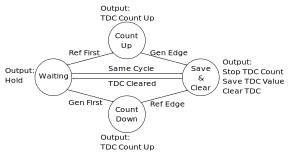
\includegraphics[width=0.8\textwidth]{../state_trans_new}
	\caption[Example State Transition Diagram for a Moore Machine]{Example State Transition Diagram for a Moore Machine.}
	\label{fig:state_trans_reprint}
\end{figure}

The synchroniser circuits are implemented by a pair of ``D'' flip-flips connected in series, clocked on the \ac{FPGA} clock. This synchroniser works by assuming that metastability will only persist for the duration of one \ac{FPGA} clock cycle as depicted in Figure \ref{fig:synchroniser_behav}. In the case where only one clock signal may experience metastability, two synchronisers are required in order to maintain symmetry in the phase comparison.
\begin{figure}[h]
\centering
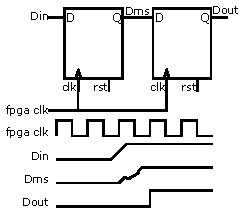
\includegraphics[width=0.4\textwidth]{../synchroniser_behav}
\caption[Double ``D'' flip-flip synchroniser circuit \ac{RTL} diagram]{Double ``D'' flip-flip synchroniser circuit \ac{RTL} diagram.}
\label{fig:synchroniser_behav}
\end{figure}

This \ac{FSM} then controls an Up-Down counter of the same width as the control code, counting in two's complement. As the control code has already been defined as a 7 bit wide two's complement integer, the phase detector's output can theoretically lie in the range $[-64,63]\cap\mathbb{Z}$. 

As this detector samples each signal at the \ac{FPGA} clock frequency, the phase detector resolution is equal to the \ac{FPGA} clock period at:
\begin{equation}
t_{res} = T_{FPGA} = \frac{1}{258\times 10^{6}} = 3.875~\si{\nano\second}
\end{equation}
an angular resolution of:
\begin{equation}
res = \frac{t_{res}}{T_{osc}} \cdot 360\si{\degree} = \frac{3.875~\si{\nano\second}}{200~\si{\nano\second}} \cdot 360\si{\degree} = 6.975\si{\degree}
\end{equation}

The counter is implemented using saturation arithmetic to prevent overflow at high phase differences which could potentially harm the ability of the \ac{ADPLL} to obtain a lock. In the case of this \ac{PD} the phase error at which overflow may occur can be computed using the bit width of the counter and temporal resolution. $error_{max} = 63\cdot3.875~\si{\nano\second} = 244.125~\si{\nano\second}$. As this is greater than the period it cannot occur for purely a phase difference, but may occur in the presence of either a frequency divider in the feedback path, thus increasing the period of the signal used for comparison, or of a significant frequency difference between the signals. When implementing the clamping logic, the decision was taken to make the detection range symmetrical, thus the output range was reduced by one increment to $[-63,63]\cap\mathbb{Z}$.

Figure \ref{fig:updown_ctr} depicts the implementation of this counter. Apart from the aforementioned capping of the measurement range implemented using a pair of comparators and a multiplexer, important to note is the bit width of the increment. Despite overflow being disallowed when the number is interpreted as a signed number, the addition of a 7 bit wide -1 to the accumulator value will cause overflow in the adder. This, however, is perfectly valid as an implementation of subtraction in two's complement. On the right side of the diagram the output register can be seen. Clocked using the \ac{FSM}s measurement interval complete signal, this register preserves the phase error until the termination of the following interval.
\begin{figure}[h]
	\centering
	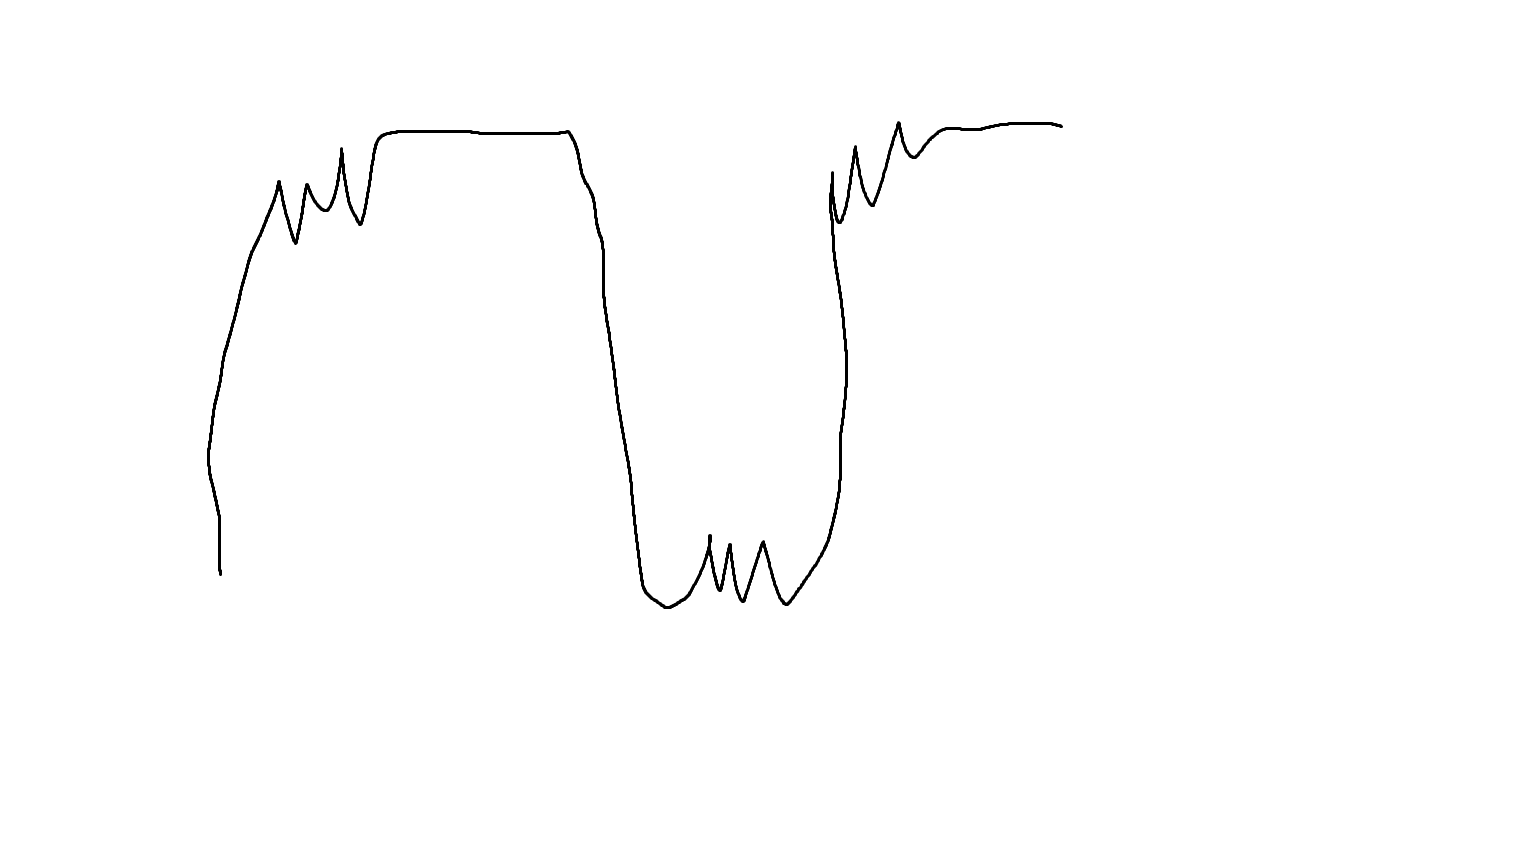
\includegraphics[width=0.6\textwidth]{../bad_waveform}
	\caption[\ac{RTL} diagram of up-down counter]{\ac{RTL} diagram of up-down counter.}
	\label{fig:updown_ctr}
\end{figure}
%TODO updown counter RTL diagram

A major pitfall was encountered in this design of phase detector, which lead in some conditions to a form of mode-locking, in which each oscillator would lock $180\si{\degree}$ phase shifted from the oscillators used as a reference. This was later discovered to be as a result of the measurement interval termination conditions in the \ac{FSM}, which in addition to those described in Figure \ref{fig:state_trans_reprint}, would terminate the interval if a falling edge was observed on the signal that originally triggered the measurement. Figure \ref{fig:uncertainty} will be used to describe the exact circumstances of the error.
\begin{figure}[h]
	\centering
	
\includegraphics[width=0.6\textwidth]{../uncertain}
	\caption[Circumstances of mode locking behaviour]{Circumstances of mode locking behaviour.}
	\label{fig:uncertainty}
\end{figure}

The situation would occur when the measurement interval began with a large phase difference between the generated and reference signals and a simultaneous difference in frequency. Without a frequency difference the measurement beginning at ``interval start'' would terminate at location ``a'', measuring a large lag, with the following measurement interval starting at location ``d''. However in the presence of a frequency differential, the rising edge on the generated signal may occur only at location ``c'', and with the falling edge termination condition causing the interval to terminate before this edge was detected, at point ``b''. This lead to a slightly lower magnitude phase lag detected, however this is a minor flaw, and not the cause of the mode locking. As the rising edge at point ``c'' occurs after the interval has terminated, it is treated as a fresh measurement interval, terminating at ``d''. As in this interval, the generated signal has seen the first rising edge, a large lead will be recorded. As each correction is made with a delay of one cycle, in order to avoid timing violations in the feedback path, there is potential for oscillation between lead and lag detection to occur depending on the initial conditions. This low probability behaviour was observed by chance, due to coding error, while using a frequency divider in the feedback path as this ensured the lead and lag measurements were of identical magnitude. 

\subsection{\acs{ADPLL} Design 2}
The second \ac{ADPLL} design implemented during the course of this project was somewhat of a stepping stone between fully synchronous and asynchronous to the \ac{FPGA} clock. The clocked phase detector is reused from above, albeit with an altered error width, while the \ac{DCO} is replaced by a \acl{RO}. While the phase detector was known to work due to testing in \ac{ADPLL} 1, the \ac{DCO} could not be simulated using accurate timings so all testing had to be done in hardware. This presented a challenge, as depending on the implementation, the characteristics of the \ac{DCO} could change, most importantly the centre frequency. 

\subsubsection{\acl{DCO}}
\ac{ADPLL} 2 exchanges the \ac{FPGA} clocked oscillator for \ac{RO}, with the aim of obtaining performance more akin to that of an \ac{ASIC} based mixed-signal implementation, due to the variation in period steps both between oscillators and within the same oscillator due to the oscillator layout. Also advantageous is the improvement in period resolution obtained using this design, when compared to that of the \ac{FPGA} clocked design. Taking the formula given in Chapter \ref{chap:3} and the inverter propagation time used by Vivado in post synthesis/implementation simulations of $315~\si{\pico\second}$, the period step can be computed:
\begin{align}
t_{step} &= \text{inverters per step}\times\text{inversions per cycle}\times\text{propagation delay} \\
t_{step} &= 2\times 2\times 315~\si{\pico\second} = 1.26~\si{\nano\second}
\end{align}
Using this period step, the number of inverters required to produce the signal of period $200~\si{\nano\second}$ can easily be computed:
\begin{equation}
\text{num\_inverters} = \left \lfloor{ T_{osc 5~\si{\mega\hertz}}}\times \frac{2}{t_{step}}}\right \rceil = \left \lfloor{ 200~\si{\nano\second}\frac{2}{1.26~\si{\nano\second}}}\right \rceil = 317
\end{equation}

Figure \ref{fig:ro_impl} contains an \ac{RTL} diagram of the \ac{RO} as implemented. %TODO impl & discuss

A control code width of 5 bits was chosen as with two inverters removed per control code, the tunable range would consist of $20\%$ of the total inverter count. To achieve this range with a centre of $317$ inverters, the maximum number of inverters in the chain was required to be $317+2\times 2^{5-1} = 349$, dropped to a minimum at $285$. The corresponding minimum and maximum frequencies then are:
\begin{align}
f_{osc} &= \frac{1}{T_{osc}} = \frac{1}{\text{num. inverters}\times\text{propagation delay}} = \frac{1}{\text{num. inverters}\0.5\timest_{step}} \\
f_{min} &= \frac{1}{T_{max}} = \frac{1}{349\times 0.5\times1.136~\si{\nano\second}} = 4.354~\si{\mega\hertz} \\
f_{max} &= \frac{1}{T_{min}} = \frac{1}{285\times 0.5\times1.136~\si{\nano\second}} = 5.332~\si{\mega\hertz}
\end{align}

The first pitfall with this type of \ac{DCO} comes in the \ac{HDL} stage, with the \ac{EDA} likely to optimise away what it sees as a long chain of inverters carrying out no function. This can be avoided by adding an \texttt{attribute} as a prefix to the instantiation of a logic element or net that should not be ``optimised'' away. It is important to choose the correct directive, otherwise the compiler may not behave as expected. In the case of Vivado, it is important not to confuse the \texttt{KEEP} or \texttt{KEEP\_HIERARCHY} commands with that of \texttt{DONT\_TOUCH}, with former commands only ensuring that the logic elements will be maintained in synthesis, but not in any subsequent stages \cite{synth_ug}.

As mentioned in previous chapters, the absence of direct control over layout can lead to significant variation of the propagation time though inverters. This may occur in three ways: Firstly, the layout of individual \ac{RO}s may be significantly different, thus resulting in poor overlap of tuning regions. Anecdotally, while implementing a 3x3 network, 7 of the 9 oscillators had centre frequencies within a $100~\si{\kilo\hertz}$ span but two lay more than $500~\si{\kilo\hertz}$ away in opposite directions which prevented the network from locking. Secondly, within an \ac{RO} the propagation delay between each inverter may vary, which results in a variable frequency step, possibly changing the locking range. These two effects represent an extreme version of the variation due to process or manufacturing seen on \ac{ASIC}s. The final variation is possibly the most frustrating, and occurs when between implementations the \ac{EDA}, Vivado in the case of this project, changes the layout of the \ac{RO}. This may occur as a result of a direct change, or as a result of seemingly innocuous changes to unrelated modules. While the final problem can be avoided, once the performance of the \ac{RO} is satisfactory, by locking down module, the remaining two problems can only be mitigated somewhat.

This is achieved by assigning specific areas of the chip in which that module must lie, although these must be of a size approximately $40\%$ larger than the minimum space required in order to avoid having the router create a complex, delay intensive layout to fit the \ac{RO}. To achieve greater consistency, the implementation directive can be modified such that the router will attempt to use the minimum area that does not require complex routing. \texttt{congestion_spreadlogic_low} was used for this purpose in this project, although other options may obtain similar results. The other options available in Vivado can be viewed in the \textit{Vivado Design Suite User Guide - Implementation} \cite{impl_ug}.

with small tweaks to unrelated modules likely to cause Vivado to rearrange the layout of the \ac{RO}s and thus change the centre frequency of a given \ac{DCO}.

\subsubsection{Phase Detector}
The \ac{PFD} used in this oscillator is, apart from the bit width of the counter, identical to that used in the previous design. The reduction in counter width will have no impact of performance of the \ac{ADPLL} once a lock has been acquired, however, the capture speed will be reduced for large phase differences due to the counter reaching saturation point significantly sooner. 5 bits corresponds to a counter range of $[-15,15]\cap\mathbb{Z}$, which will saturate at a time delay of $15\times3.875\si{\nano\second} = 58.125~\si{\nano\second}$, a phase lead or lag of $\frac{}{}\times360\si{\degree} = 104.4\si{\degree}$ at $5~\si{\mega\hertz}$. This is an adequate range, as saturation will occur well outside of the normal operating range. This reduction is most noticeable when a divider is active in the feedback path, however during locked operation a phase shift of $58.125~\si{\nano\second}$ will not occur, so this impact is only felt during acquisition.

\subsection{\acs{ADPLL} Design 3}
\subsubsection{\acl{DCO}}
\subsubsection{Phase Detector}


\section{\acs{ADPLL} Characterisation}

\section{Minor Variations}\label{section:minor_variations}
%TODO osc side

\section{\acs{ADPLL} Network Implementation}
\subsection{2x2 Network}
\subsection{3x3 Network}
